% Real-time VJF with an unknown observation model.
% catniplab.sty + math_preamble.tex are resolved via TEXINPUTS (see Makefile/.envrc);
% do not vendor them. Notation follows Zhao & Park (2020).
\documentclass[11pt]{article}
\usepackage[preprint]{catniplab}
\input{math_preamble}

\usepackage{graphicx}
\usepackage{booktabs}
\usepackage{cleveref}

% extras not provided by math_preamble (which auto-defines \va..\vz, \vA..\vZ, \vphi)
\newcommand{\E}{\mathbb{E}}
\newcommand{\vmu}{\bm{\mu}}
\newcommand{\vnu}{\bm{\nu}}
\newcommand{\vpi}{\bm{\pi}}
\newcommand{\vSig}{\bm{\Sigma}}
\newcommand{\veps}{\bm{\epsilon}}

\addbibresource{references.bib}

\title{Real-time variational joint filtering of neural dynamics\\ with an unknown observation model}
\author{I.~Memming Park}
\date{\today}

\begin{document}
\maketitle

\begin{abstract}
Variational joint filtering (VJF) learns a latent nonlinear dynamical system and infers its
state online, one observation at a time, making it attractive for closed-loop neuroscience.
In practice two obstacles remain: the observation (readout) model is rarely known a priori, and
naively estimating it by gradient descent on the variational objective collapses to a trivial
mean-rate solution under sparse, low-rate spikes. We present a real-time extension of VJF that
(i) feeds the recognition network a low-dimensional \emph{subspace projection} of the
observations rather than the raw spikes, (ii) estimates the readout \emph{online and decoupled
from the variational gradient} by incremental PCA with an orthogonal-Procrustes anchor, and
(iii) stabilizes the dynamics fit over long streams with a square-root recursive least squares
flow learner. The generative model and the filtering objective are unchanged. On a 1000\,s
biologically calibrated Poisson limit-cycle benchmark the method runs in $\sim$3\,ms per 5\,ms
bin (real-time, single CPU) and, with an \emph{unknown} readout, recovers the latent dynamics;
the projection encoder is a clear and robust win at fixed readout, while the online readout
comes within $0.02$ of the known-readout ceiling at low SNR and trails it at high SNR --- an effect we trace to
the frame motion induced by periodic readout refresh, and which we leave as an open problem.
\end{abstract}

\section{Introduction}
Inferring low-dimensional latent dynamics from neural population spiking, \emph{as the data
arrive}, is the core requirement of closed-loop experiments and adaptive brain--machine
interfaces. Variational joint filtering \autocite{zhao2020variational} meets the streaming
requirement: it couples an amortized recognition network \autocite{kingma2014auto} with a
recursive estimate of a nonlinear state-space model, updating both the posterior and the model
parameters once per time bin. Two issues stand between VJF and a turnkey real-time tool. First,
the observation model --- the loading matrix $\vC$ and bias $\vb$ mapping latents to firing
rates --- is typically unknown and must be learned from the same stream; under sparse, low-rate
Poisson spikes the gradient of the variational objective with respect to $\vC$ is scaled by the
per-bin rate ($\sim 10^{-1}$) and the fit collapses to ``explain the mean rate through $\vb$.''
Second, the correct streaming control flow (posterior threading, a warm-up before the dynamics
are turned on, divergence guards, numerically stable recursive updates) is subtle and, in
released code, lives only inside experiment scripts.

We address all three. \Cref{sec:method} introduces a \emph{projection-input recognition} that
hands the network the readout's own approximate inverse, a \emph{decoupled online readout}
estimated by incremental PCA rather than by the variational gradient, and a \emph{square-root
RLS} dynamics learner for long-stream stability; we also package the streaming loop as a
reusable per-sample primitive. Throughout we keep the generative model and the filtering
objective of \autocite{zhao2020variational} unchanged, and we emphasize precisely \emph{what
differs} from vanilla VJF. \Cref{sec:exp,sec:results} validate the method on a 1000\,s
biologically calibrated Poisson limit cycle and report an honest, mixed picture.

\section{Background: variational joint filtering}\label{sec:bg}
With latent $\vx_t\in\reals^m$, observation $\vy_t\in\reals^n$, and optional input $\vu_t$, VJF
assumes a point-process / GLM observation and an additive radial-basis-function (RBF) dynamics,
\begin{align}
  \vy_t &\sim P\!\big(g(\vC\vx_t+\vb)\big), \qquad g=\exp, \tag{lik}\label{eq:lik}\\
  \vx_{t+1} &= \vx_t + f(\vx_t) + \vB_t\vu_t + \veps_{t+1},\quad
  f(\vx)=\vW\vphi(\vx),\quad \veps_t\sim\mathcal N(\bm0,\sigma^2\vI). \tag{gen}\label{eq:gen}
\end{align}
A recognition network $h$ produces the recursive Gaussian posterior $q(\vx_t)=\mathcal
N(\vmu_t,\vs_t)$ (with $\vs_t$ the per-dimension variance), and all parameters are learned by
maximizing the per-step filtering ELBO (with $\tilde\vx_t$ a reparameterized sample from $q(\vx_t)$),
\begin{align}
  [\vmu_t,\vs_t] &= h(\vy_t,\vu_{t-1},\vmu_{t-1},\vs_{t-1}), \tag{recog}\label{eq:recog}\\
  \hat{\mathcal L} &= \log p(\vy_t\mid\tilde\vx_t,\theta)
     + \E_{q(\vx_t)}\log p(\vx_t\mid\tilde\vx_{t-1},\theta) + H(q(\vx_t)). \tag{ELBO}\label{eq:elbo}
\end{align}
The observation model is identifiable only up to an invertible $\vR$, since
$\vC\vx_t=(\vC\vR)(\vR^{-1}\vx_t)$; \autocite{zhao2020variational} initializes $\vC$ by factor
analysis and \emph{column-wise $\ell_2$-normalizes} it every iteration, which fixes the column
scale but leaves the rotation/reflection free.

\section{Method}\label{sec:method}
We make three coupled changes (\cref{ssec:proj,ssec:readout,ssec:srrls}); the generative model
\cref{eq:lik,eq:gen} and the objective \cref{eq:elbo} are untouched. Vanilla VJF is recovered by
setting $\vpi_t:=\vy_t$ and learning $\vC$ by $\partial\hat{\mathcal L}/\partial\vC$.

\subsection{Projection-input recognition}\label{ssec:proj}
The recognition map \cref{eq:recog} must invert $n$ sparse channels into $m$ latent dimensions,
which is hard to learn at low SNR. We replace the raw observation by a deterministic,
$\vC$-dependent feature: the least-squares projection of a link-matched observation feature onto
the current loading subspace,
\begin{align}
  \vpi_t &= \vC^{+}\,(\tilde g(\vy_t)-\vb),\qquad
     \vC^{+}\in\reals^{m\times n}\ \text{the Moore--Penrose pseudoinverse}, \label{eq:proj}\\
  [\vmu_t,\vs_t] &= h(\vpi_t,\vu_{t-1},\vmu_{t-1},\vs_{t-1}). \tag{recog$'$}
\end{align}
($\vC^{+}=(\vC\trp\vC)^{-1}\vC\trp$ when $\vC$ has full column rank.)
Here $\tilde g$ is a variance-stabilizing, approximate inverse link. For the point-process case
$\tilde g(\vy_t)=\log(\vnu_t+c)$ with a causal exponential moving average (EMA) of the counts,
\begin{equation}
  \vnu_t = (1-\alpha)\,\vnu_{t-1}+\alpha\,\vy_t,\qquad \alpha=1/\tau, \tag{EMA}\label{eq:ema}
\end{equation}
(memory $\sim\tau$ bins; $\tau{=}1$ disables smoothing), and $\tilde g=\mathrm{id}$ for Gaussian
observations. \textbf{Difference from VJF:} the recognition input shrinks from $\reals^n$ to
$\reals^m$ with $m\!\ll\!n$, so the network never sees the raw, high-dimensional, sparse spike
vector --- only its $m$-dimensional subspace coordinate, the readout's own approximate inverse.
The network then need only perform an $m\!\to\!m$ correction. Because $q(\vx_t)$ may be any
data-dependent distribution, parameterizing it through $\vpi_t$ leaves the bound
\cref{eq:elbo} valid; only the amortization family changes. $\vC^{+}$ is recomputed only when
$\vC$ is refreshed (\cref{ssec:readout}) and reused as one $O(nm)$ map per bin. The timescale
$\tau$ is a fixed hyperparameter ($\tau\ll$ the dynamics timescale), not ELBO-learned.

\subsection{Decoupled online readout estimation}\label{ssec:readout}
Estimating $\vC$ by $\partial\hat{\mathcal L}/\partial\vC$ under sparse low-rate Poisson
collapses to the trivial mean-rate solution: the gradient is scaled by the per-bin rate
$g(\vC\vx_t+\vb)\!\approx\!10^{-1}$, so $\vC$ barely moves and a basin with $\vC\!\to\!0$
absorbs the loss. \textbf{Difference from VJF:} we replace this gradient by a \emph{decoupled}
online second-moment estimator. Let $\vl_t=\tilde g(\vy_t)$ and $\bar\vb_t$ its running mean
(which serves as $\vb$). We track the top-$m$ subspace of the centered feature
$\vr_t=\vl_t-\bar\vb_t$ (distinct from the control $\vu_t$) by candid covariance-free
incremental PCA (CCIPCA) \autocite{weng2003candid}: maintaining vectors $\vv_1,\dots,\vv_m$ that
converge to $\lambda_i\ve_i$ (eigenvalue $\times$ eigenvector of $\E[\vr\vr\trp]$) without ever
forming that matrix. With $\vr_t^{(1)}=\vr_t$ and rate $\eta_t=1/t$, for $i=1,\dots,m$,
\begin{align}
  \vv_i &\leftarrow (1-\eta_t)\,\vv_i + \eta_t\,\big(\vr_t^{(i)\trp}\hat\vv_i\big)\,\vr_t^{(i)},
     \qquad \hat\vv_i=\vv_i/\norm{\vv_i}, \tag{Hebb}\label{eq:hebb}\\
  \vr_t^{(i+1)} &= \vr_t^{(i)} - \big(\vr_t^{(i)\trp}\hat\vv_i\big)\,\hat\vv_i. \tag{deflate}\label{eq:deflate}
\end{align}
Each component is an online power iteration on the covariance
($\E[(\vr\trp\hat\vv_i)\vr]=\E[\vr\vr\trp]\hat\vv_i$) followed by Gram--Schmidt deflation so that
component $i{+}1$ sees only the orthogonal complement. At convergence $\norm{\vv_i}=\lambda_i$
and the loading column is $\vc_i=\hat\vv_i\sqrt{\norm{\vv_i}}=\ve_i\sqrt{\lambda_i}$ (unit-variance
latent). This is a well-conditioned M-step, free of the rate-scaled-gradient collapse, and
shared by the decoder \cref{eq:lik} and the projection \cref{eq:proj}; it is a streaming analogue
of the PLDS/GPFA-style readout warm-start \autocite{macke2011empirical,yu2009gaussian}. The
estimate $\hat\vC_t$ is written to the decoder every $K$ steps.

\paragraph{Identifiability / normalization.}
The column-$\ell_2$ normalization of \autocite{zhao2020variational} fixes only the scale gauge.
Our setting needs more: each incremental-PCA refresh returns a basis with an arbitrary rotation
and sign (eigenvectors are signed; near-degenerate eigenvalues rotate freely). We therefore fix
the full orthogonal gauge by orthogonal Procrustes alignment of the refreshed loading to the
previous one,
\begin{equation}
  \vR^\star=\arg\min_{\vR\trp\vR=\vI}\norm{\hat\vC\vR-\vC_{\mathrm{prev}}}_F=\vU\vV\trp,\qquad
  \hat\vC\trp\vC_{\mathrm{prev}}=\vU\vSig\vV\trp\ (\text{SVD}), \label{eq:procrustes}
\end{equation}
and fix the scale by the unit-variance column scaling above. This removes the sign/rotation
jumps between refreshes and keeps the latent frame approximately fixed; the residual frame
motion, and its effect on the learned dynamics $f=\vW\vphi$, is taken up in \cref{sec:discussion}.

\subsection{Square-root RLS dynamics and the real-time loop}\label{ssec:srrls}
Over a long online pass the recursive least-squares (RLS) fit of the RBF velocity weights
accumulates error in the precision matrix and eventually diverges. \textbf{Difference from VJF:}
we propagate a covariance square-root factor $\vS$ ($\vP=\vS\vS\trp$) directly (square-root RLS,
\autocite{haykin2014adaptive,schoenberg1983implementation}), avoiding the precision wind-up that
destabilizes plain RLS over long ($\sim2\times10^5$-step) streams; stochastic-gradient flow is
stable but slower to converge. Finally, the
streaming control flow --- posterior threading, a warm-up phase during which the dynamics are
frozen while the recognition settles (followed by a one-time initialization of $f$ from the
buffered latent means and a narrowing of the RBF widths), divergence recovery (a state-noise
floor and repeat-last-state), the projection wiring, the periodic Procrustes refresh, and
per-bin timing --- is encapsulated as a single per-sample generator, so a real-time consumer
calls one function per arriving sample. The projection and readout add $O(nm)$ per step (the same
order as the decoder); the total per-step cost also includes the recognition network and the
RBF / square-root-RLS update.

\section{Experiments}\label{sec:exp}
We use a self-contained synthetic benchmark: a 2-D limit cycle (radius-relaxing, constant
angular velocity) observed through a sparse log-linear Poisson population, calibrated to
biological rates (mean $\sim20$\,Hz, peak $\le100$\,Hz at 5\,ms bins). One single-trial stream
of $T=200{,}000$ bins (1000\,s) is generated; signal-to-noise is set by population size, giving
three conditions ($n=50/150/250$ neurons, $\sim3/6/8$\,dB). \Cref{fig:raster} shows the input.
We compare five configurations, crossing the \emph{recognition input} (spike vs.\ projection)
with how the \emph{readout} is obtained (oracle = true $\vC$; online $\hat\vC_t$ from
\cref{ssec:readout}; or a frozen batch-PCA readout from a $60n$-bin window):
spike+oracle (the raw-VJF bound), projection+oracle (the projection ceiling),
projection+online ($\tau{=}8$ and $\tau{=}1$), and spike+frozen-PCA. The dynamics use
square-root RLS throughout. We report the filtered-latent $R^2$ (best affine image of the
posterior mean vs.\ the true latent), one-step prediction $R^2$, rate correlation, free-run
forecast horizon, and the steady per-bin compute time.

\begin{figure}[t]
\centering
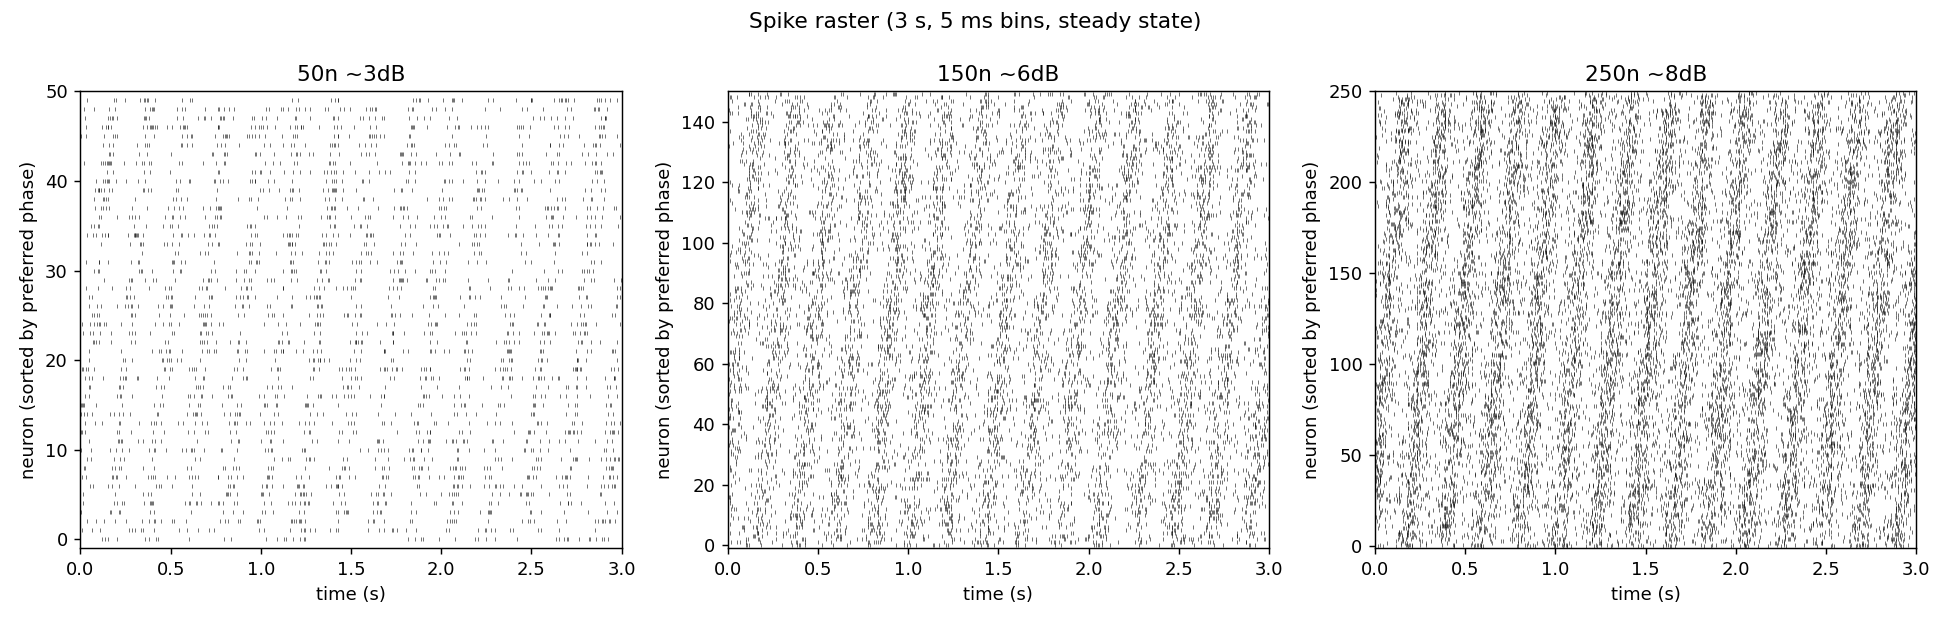
\includegraphics[width=\textwidth]{figs/raster.png}
\caption{Example input: 3\,s spike rasters (neurons sorted by preferred phase) at the three SNR
levels. The rotational structure is barely visible at $n{=}50$ and sharp at $n{=}250$.}
\label{fig:raster}
\end{figure}

\section{Results}\label{sec:results}
\Cref{tab:r2} and \cref{fig:summary} give the filtered-latent $R^2$. Three points stand out, and
the picture is honestly mixed.

\begin{table}[t]
\centering
\caption{Filtered-latent $R^2$ (best affine image of the posterior mean vs.\ truth). The ceiling
is projection+oracle; \textbf{bold} marks the best \emph{achievable} (non-oracle) method per SNR.}
\label{tab:r2}
\begin{tabular}{lccc}
\toprule
recognition input / readout & $3$\,dB & $6$\,dB & $8$\,dB\\
\midrule
proj.\ enc., oracle $\vC$ (ceiling)          & 0.86 & 0.94 & 0.96\\
spike enc., oracle $\vC$ (raw-VJF bound)      & 0.69 & 0.84 & 0.91\\
proj.\ enc., online $\hat\vC_t$ ($\tau{=}8$)  & \textbf{0.84} & 0.86 & 0.85\\
proj.\ enc., online $\hat\vC_t$ ($\tau{=}1$)  & 0.73 & 0.84 & 0.88\\
spike enc., frozen PCA $\vC$                   & 0.72 & \textbf{0.87} & \textbf{0.92}\\
\bottomrule
\end{tabular}
\end{table}

\textbf{(1) The projection input is a clear, robust win at fixed $\vC$.} Projection+oracle beats
spike+oracle at every SNR, most strongly on one-step prediction ($0.84/0.95/0.97$ vs.\
$0.60/0.85/0.92$): feeding $\vpi_t=\vC^{+}(\tilde g(\vy_t)-\vb)$ spares the network the
$n\!\to\!m$ inversion and the high-dimensional sparse input.
\textbf{(2) The online readout reaches the ceiling, in filtered-latent $R^2$, only at low SNR.}
At $3$\,dB the online estimate comes within $0.02$ of the projection ceiling ($0.84$ vs.\
$0.86$; and well above frozen-PCA $0.72$ and spike-oracle $0.69$) --- though even there it does
not lead on one-step prediction or forecast horizon; at $8$\,dB it trails
even a well-initialized frozen PCA ($0.85$ vs.\ $0.92$) and its own oracle ceiling. The periodic
Procrustes refresh keeps moving the latent frame, so the dynamics fit a moving target: online
one-step $R^2$ ($0.58/0.71/0.71$) and forecast horizon ($k{=}11/82/100$; \cref{fig:kstep}) trail
the fixed-$\vC$ modes (\cref{fig:curves} shows the online estimate still climbing at $1000$\,s
for high SNR).
\textbf{(3) Smoothing helps the noisy regime and rate fidelity.} Rate correlation is
$0.84/0.88/0.87$ at $\tau{=}8$ vs.\ $0.54/0.71/0.76$ at $\tau{=}1$; the EMA denoises the readout
feature at the cost of a small lag that mildly reduces high-SNR latent $R^2$.

Per-bin online cost is flat at $\sim3$\,ms ($50\!\to\!250$ neurons) on a single CPU core --- i.e.\
real-time at $5$\,ms bins, closed-loop feasible --- with zero divergences over the $1000$\,s pass.
At good SNR the learned flow forecasts $\sim2.4$ cycles ahead ($k{=}100$; \cref{fig:forecast}).

\begin{figure}[t]
\centering
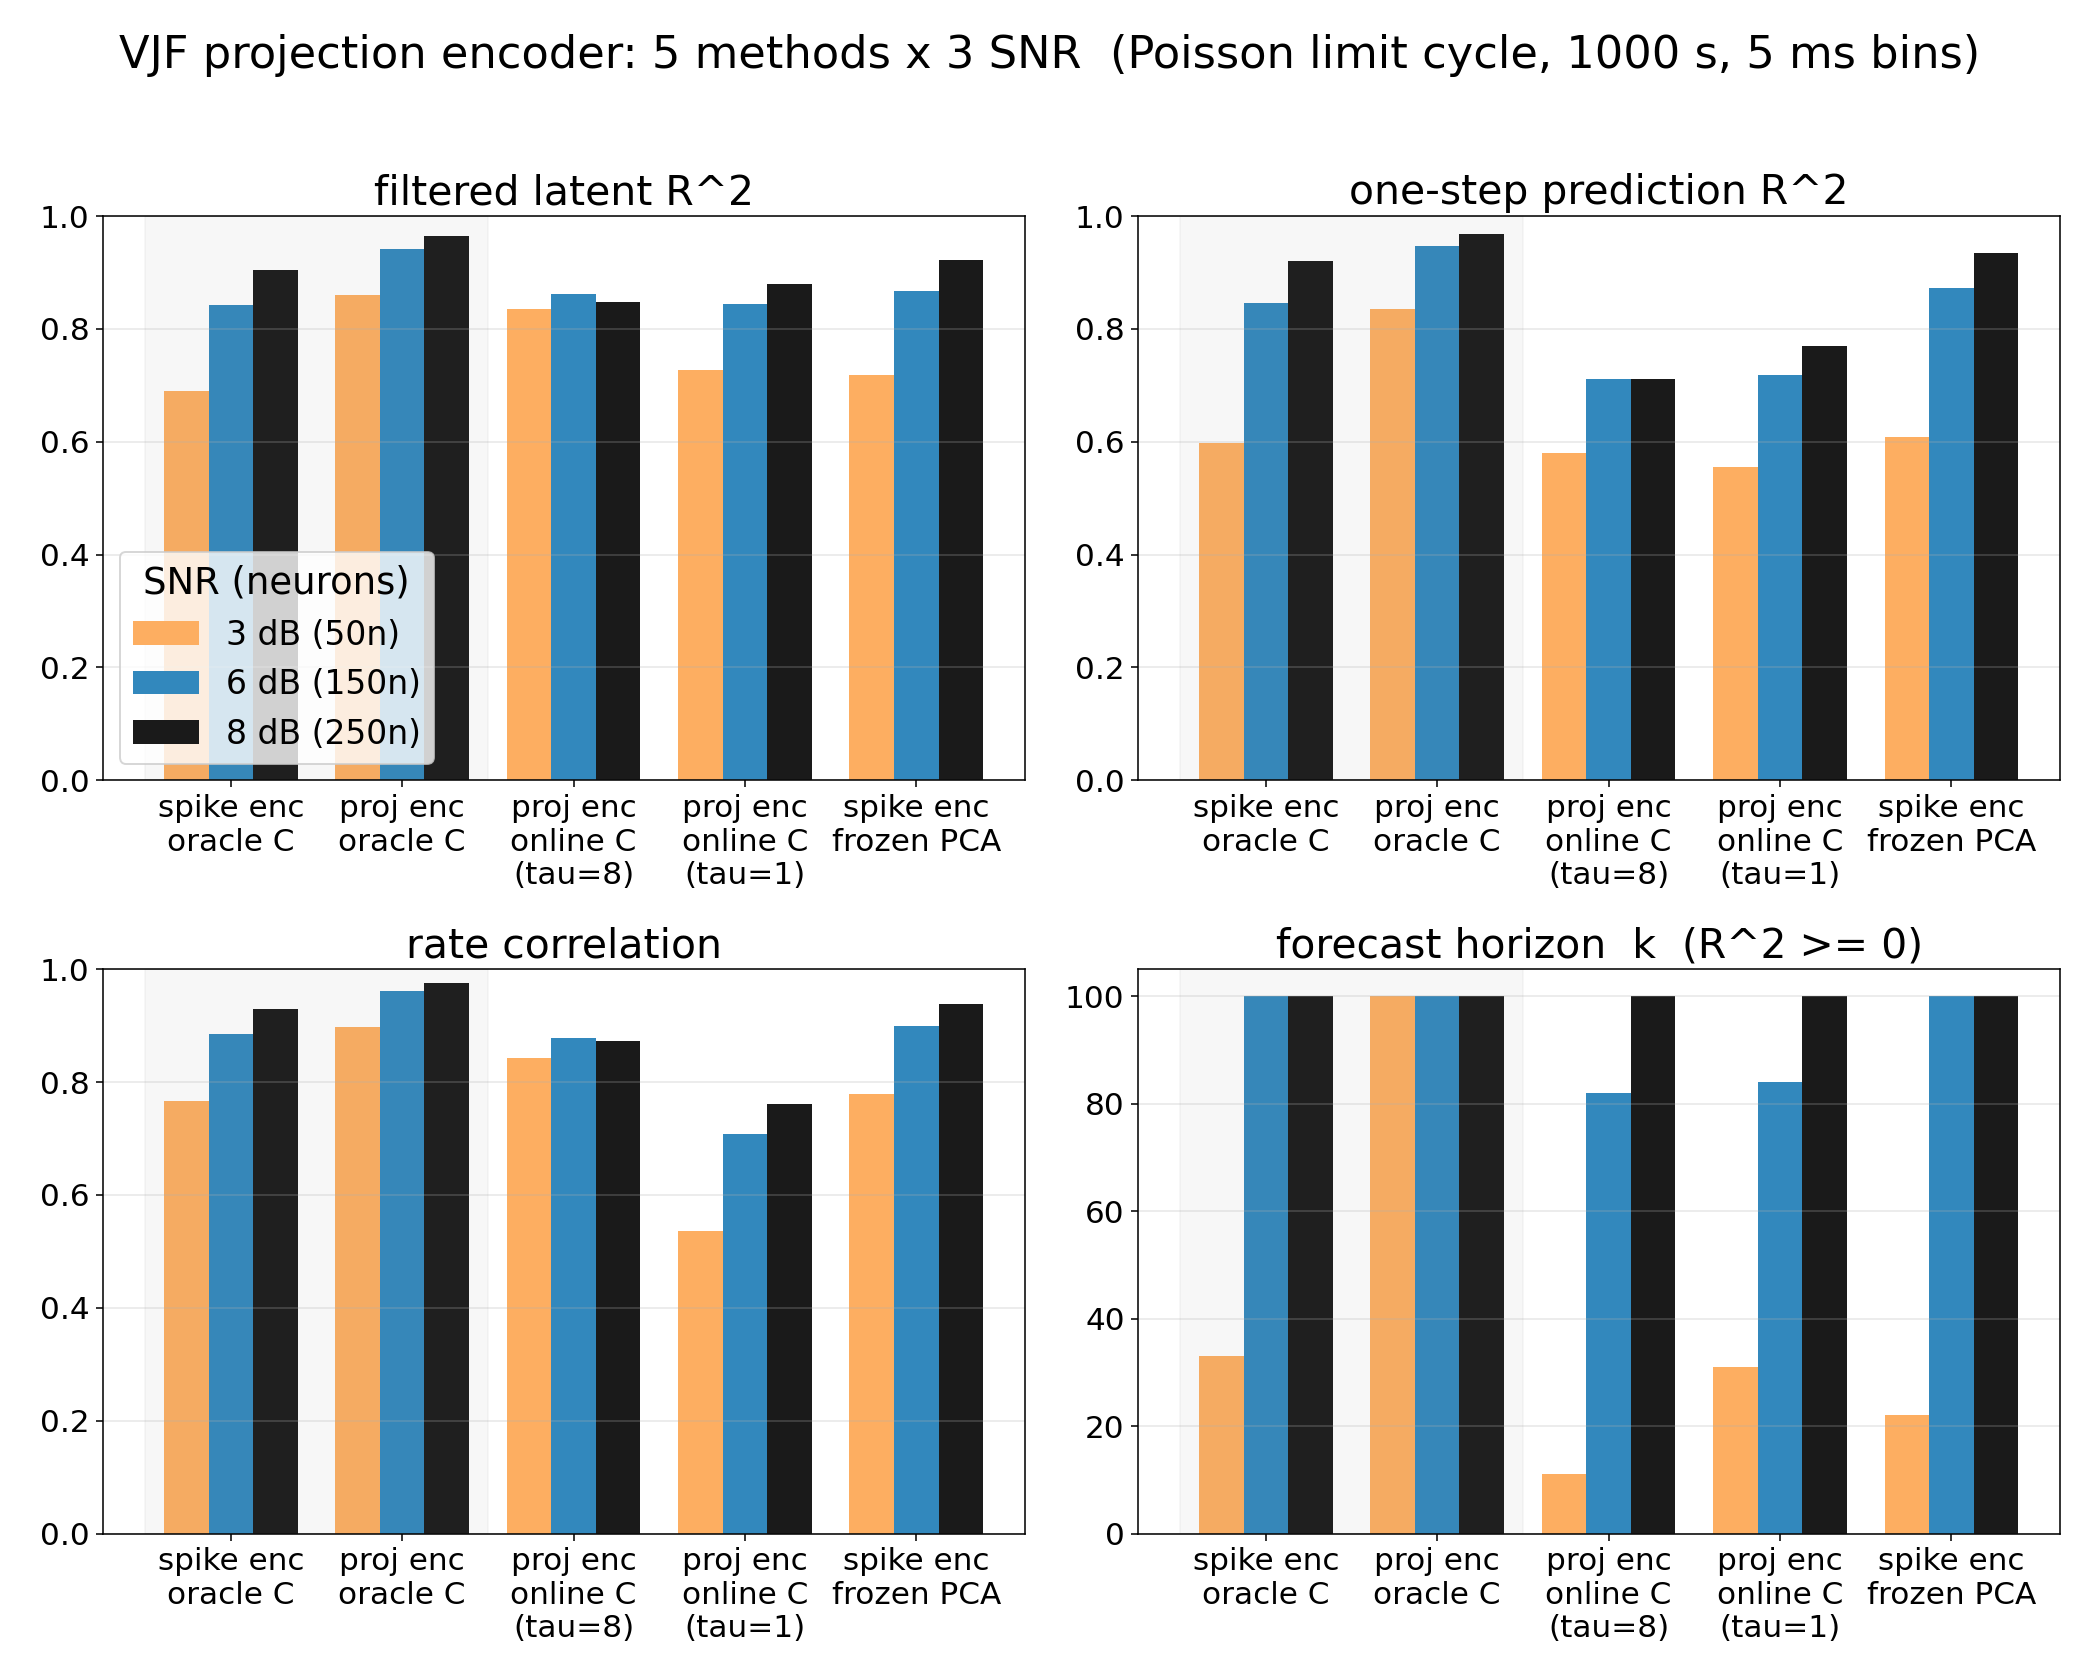
\includegraphics[width=\textwidth]{figs/summary.png}
\caption{Headline metrics, grouped by method ($x$-axis), three SNR bars each. Projection+oracle
(the ceiling) dominates; the online readout matches it only at $3$\,dB and trails on one-step
prediction and forecast horizon at higher SNR.}
\label{fig:summary}
\end{figure}

\begin{figure}[t]
\centering
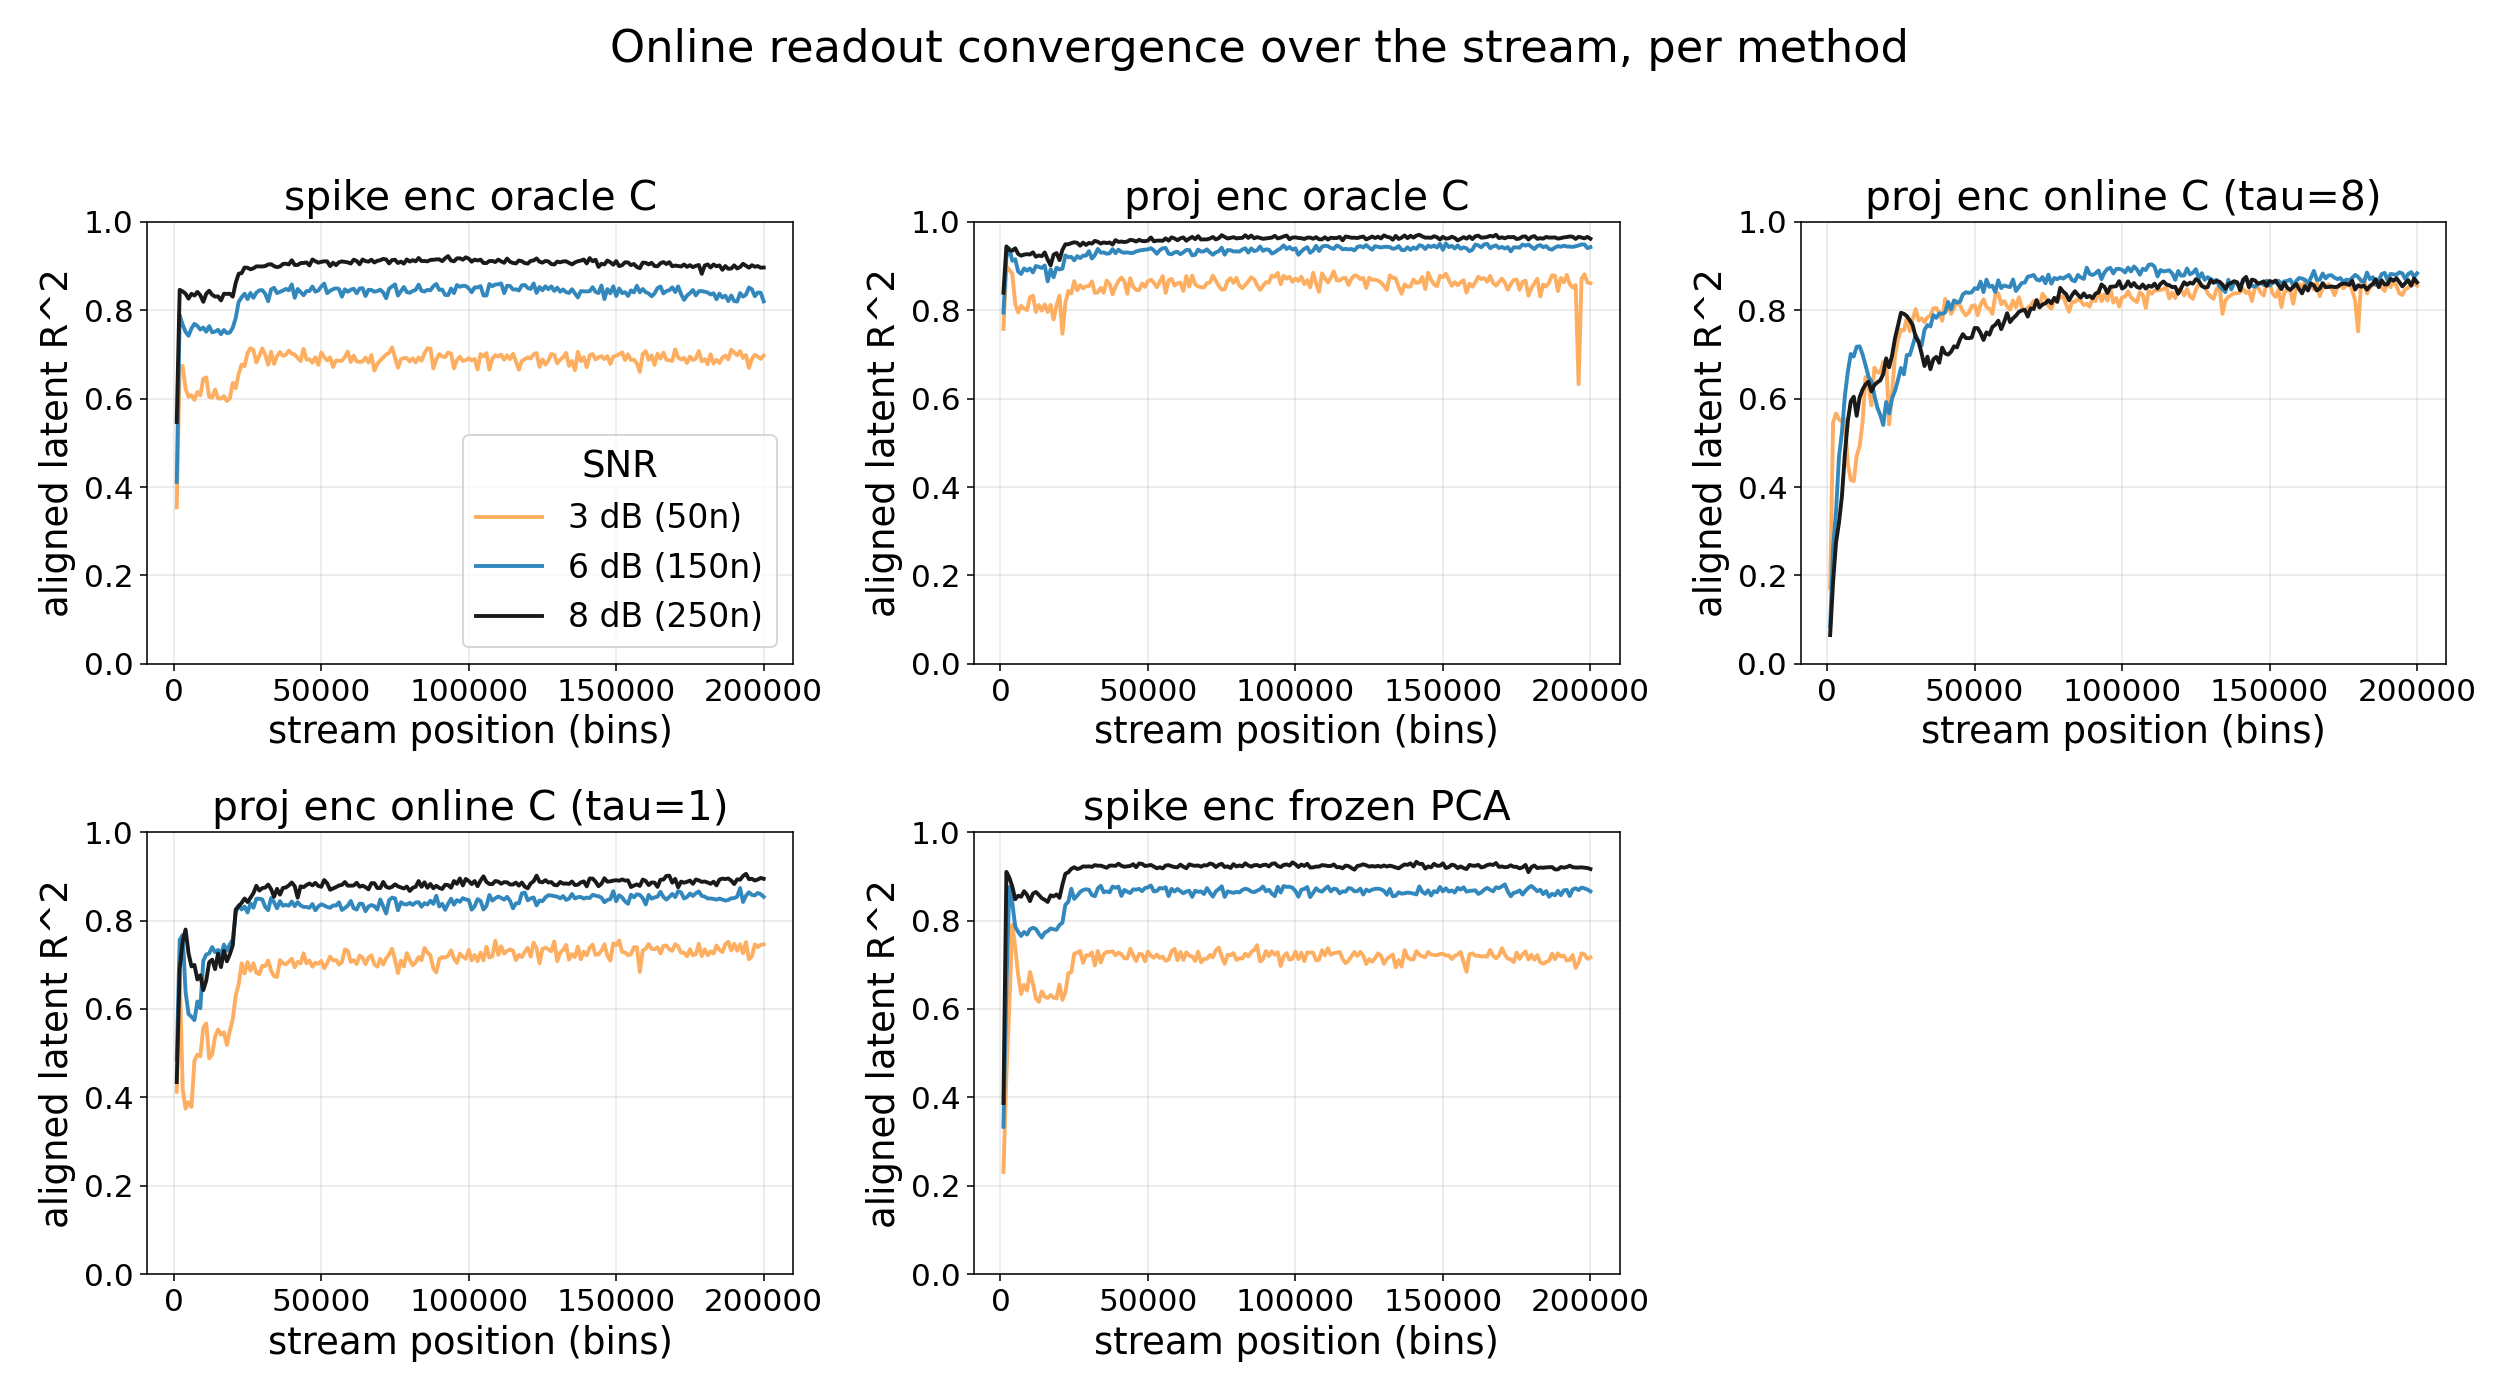
\includegraphics[width=\textwidth]{figs/curves.png}
\caption{Aligned latent $R^2$ over the $1000$\,s stream, one panel per method, one curve per SNR.
Fixed-$\vC$ methods lock in early in the stream; the online estimate ($\tau{=}8$, top right)
rises slowly and at $8$\,dB is still climbing at $1000$\,s --- the high-SNR shortfall of
\cref{tab:r2}.}
\label{fig:curves}
\end{figure}

\begin{figure}[t]
\centering
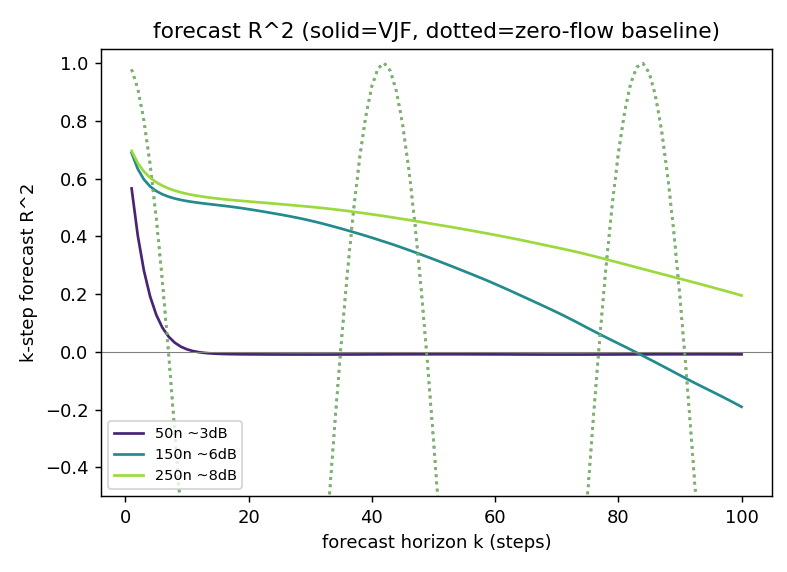
\includegraphics[width=0.72\textwidth]{figs/kstep.png}
\caption{$k$-step free-run forecast $R^2$ of the final online model (solid) vs.\ a zero-flow
baseline (dotted, which oscillates as the periodic orbit returns near its start every $\sim42$
bins). Skill holds to $k\!\approx\!82/100$ at $6/8$\,dB and decays by $k\!\approx\!12$ at
$3$\,dB.}
\label{fig:kstep}
\end{figure}

\begin{figure}[t]
\centering

\includegraphics[width=\textwidth]{figs/forecast.png}
\caption{Single-trial $100$-step free-run forecasts of the online model (dashed; $\circ=$ start)
vs.\ the true trajectory (solid). At $6/8$\,dB the learned flow tracks the cycle, though some
runs relax onto a slightly smaller orbit (the learned attractor); at $3$\,dB the forecast
degrades quickly (horizon $k\!\approx\!12$, \cref{fig:kstep}). The smaller-orbit relaxation is the
frame-churn effect that caps high-SNR one-step accuracy.}
\label{fig:forecast}
\end{figure}

\section{Discussion}\label{sec:discussion}
With an unknown observation model, real-time VJF is feasible: a cheap small-window readout
warm-start plus the projection encoder recovers the latent dynamics online at biological rates
and real-time cost, and the projection encoder is a robust, SNR-graded improvement over
raw-spike recognition even when $\vC$ is known. The remaining gap is the online readout at high
SNR, where it does not reach its own (projection-oracle) ceiling and is beaten by a frozen
batch-PCA readout. The mechanism is the periodic Procrustes refresh: each rewrite of $\vC$ shifts
the latent coordinate frame, and the recursive dynamics learner must chase a moving target,
degrading one-step prediction and forecast horizon even when instantaneous filtering is accurate.
Promising remedies, left as future work, are to anneal or freeze the refresh once the subspace
stabilizes, or to rotate the RBF flow by $\vR^\star$ at each refresh (exact for a rotation: the RBF centers
$\bm{\xi}_i\mapsto\vR^\star\bm{\xi}_i$, with $\vW$ transformed accordingly) so the dynamics track
the frame.

\printbibliography

\end{document}
